\section{Kubernetes Object Management}
The imperative approach would start single pods or services using pods from the command line:

\emph{``Create new application pod!''} \\
The declarative approach applies configure files to update the current state:

\emph{``I want a deployment with 5 application pods..''}

\vspace{3mm}
\noindent
General commands to use for different kinds of resources:

\vspace{3mm}
\ttfamily
\noindent
kubectl get \emph{pods}\rmfamily

display basic information about a resource type

\ttfamily
\noindent
kubectl describe \emph{pod} pod-name\rmfamily

get detailed information about a specific resource entity

\ttfamily
\noindent
kubectl get \emph{pods} -o wide \rmfamily

display more information

\ttfamily
\noindent
kubectl get \emph{pod} pod-name -o yaml \rmfamily

display config of a running entity in yaml format

\ttfamily
\noindent
kubectl explain \emph{pod.spec}\rmfamily

\begin{figure}[h]
    \centering
    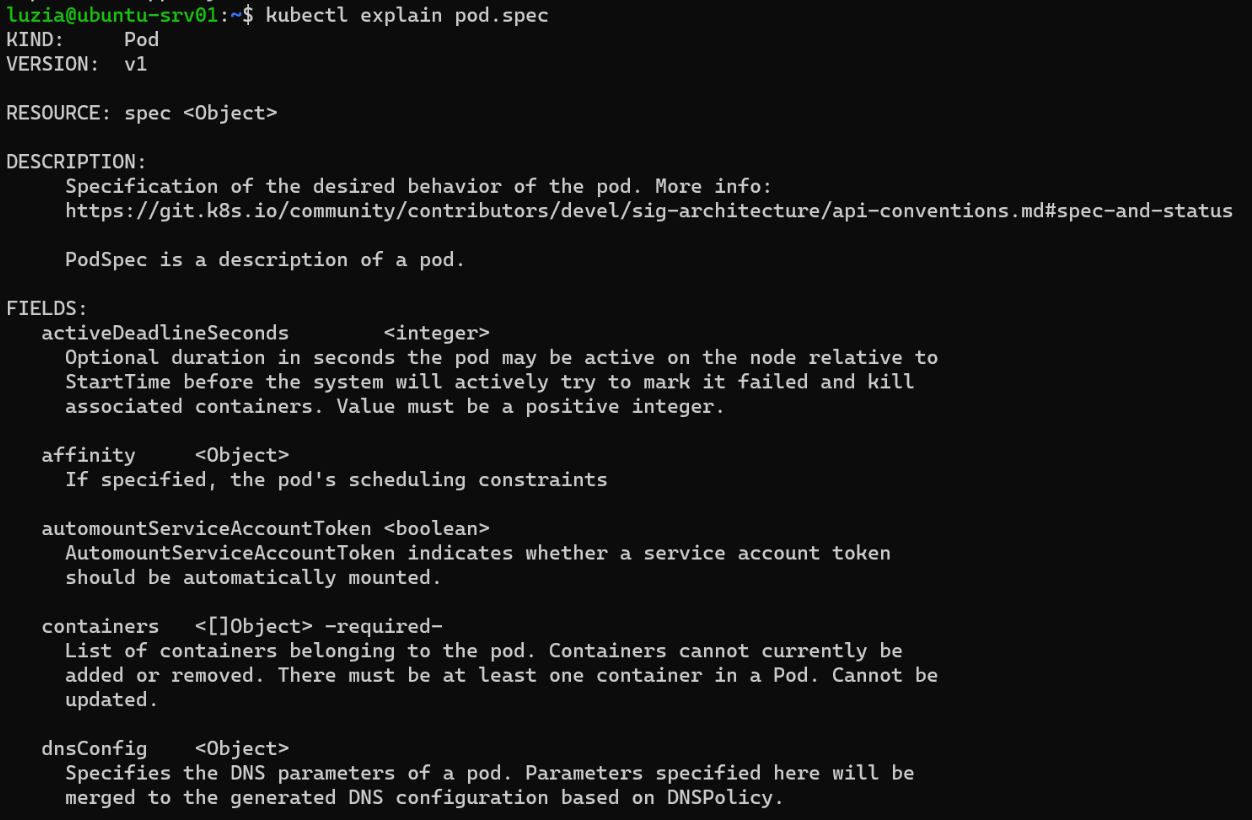
\includegraphics[width=\textwidth]{kubernetes-explain-podspec}
    \caption{Detailed Spec Information for Resource Types}
\end{figure}

\subsection{Pods and Containers}
A pod is an abstraction of a server. It usually runs one container performing some service, as well as sidecar containers 
performing additional networking or logging tasks like monitoring or service mesh functionality.

A pod is the minimal entity managed by Kubernetes. Typically only started within a deployment to ensure fault-tolerance.

\begin{figure}[h]
    \centering
    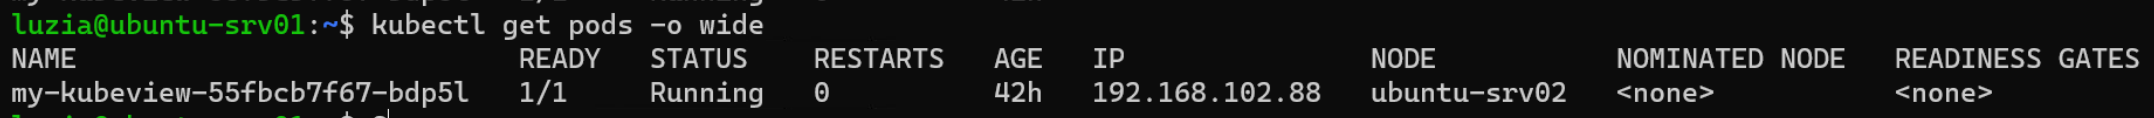
\includegraphics[width=\textwidth]{kube-get-pods.png}
    \caption{Get Pod Information}
\end{figure}

\noindent
Configure pods with the following metadata

\ttfamily
apiVersion:

kind:

metadata:

spec:
\rmfamily

\vspace{3mm}
\noindent
Connecting to a pod for further inspection:

\ttfamily
    kubectl exec -it \emph{pod-name} -- \emph{command}
\rmfamily

\subsubsection{Sidecar Container}
Runs services like monitoring that are able to directly access the main container inside a pod.

\subsubsection{Init Container}
Container which is started to complete a job before the pods main container starts. 
If this job fails, the main container is not started. 


\subsection{Namespaces}
A namespace implements linux kernel level resource isolation. Can be used to strictly separate between customer resources.

Set current namespace: 

\noindent
\ttfamily kubectl config set-context --current --namespace==\emph{name}\rmfamily

\subsection{Resource Limitations}
By default, pods use as much resources as they need. Resource limits can be defined inside the pod specifications.

\begin{figure}[h]
    \centering
    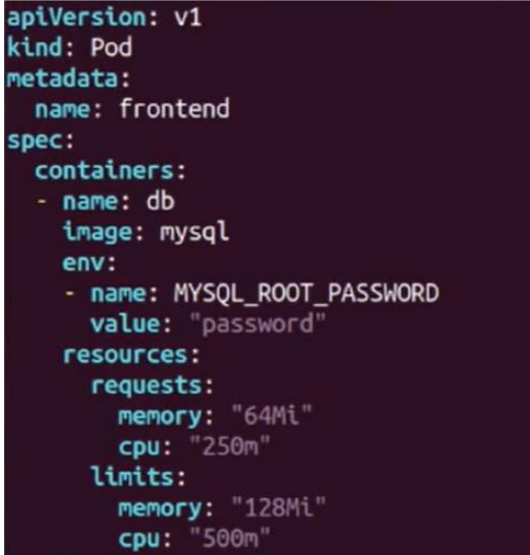
\includegraphics[width=5cm]{kubernetes-pod-resourcelimits.png}
    \caption{Pod Resource Limits}
\end{figure}

\subsection{Deployments}
Adds additional features to single pod deployments, like scalability and update strategies. 

Deployments create and manage ReplicaSets to ensure a stable set of identical pods running at any given time. 

Check deployment rollout status using the following command:

\ttfamily
kubectl rollout status deployment/\emph{deployment-name}
\rmfamily

\begin{figure}[h]
    \centering
    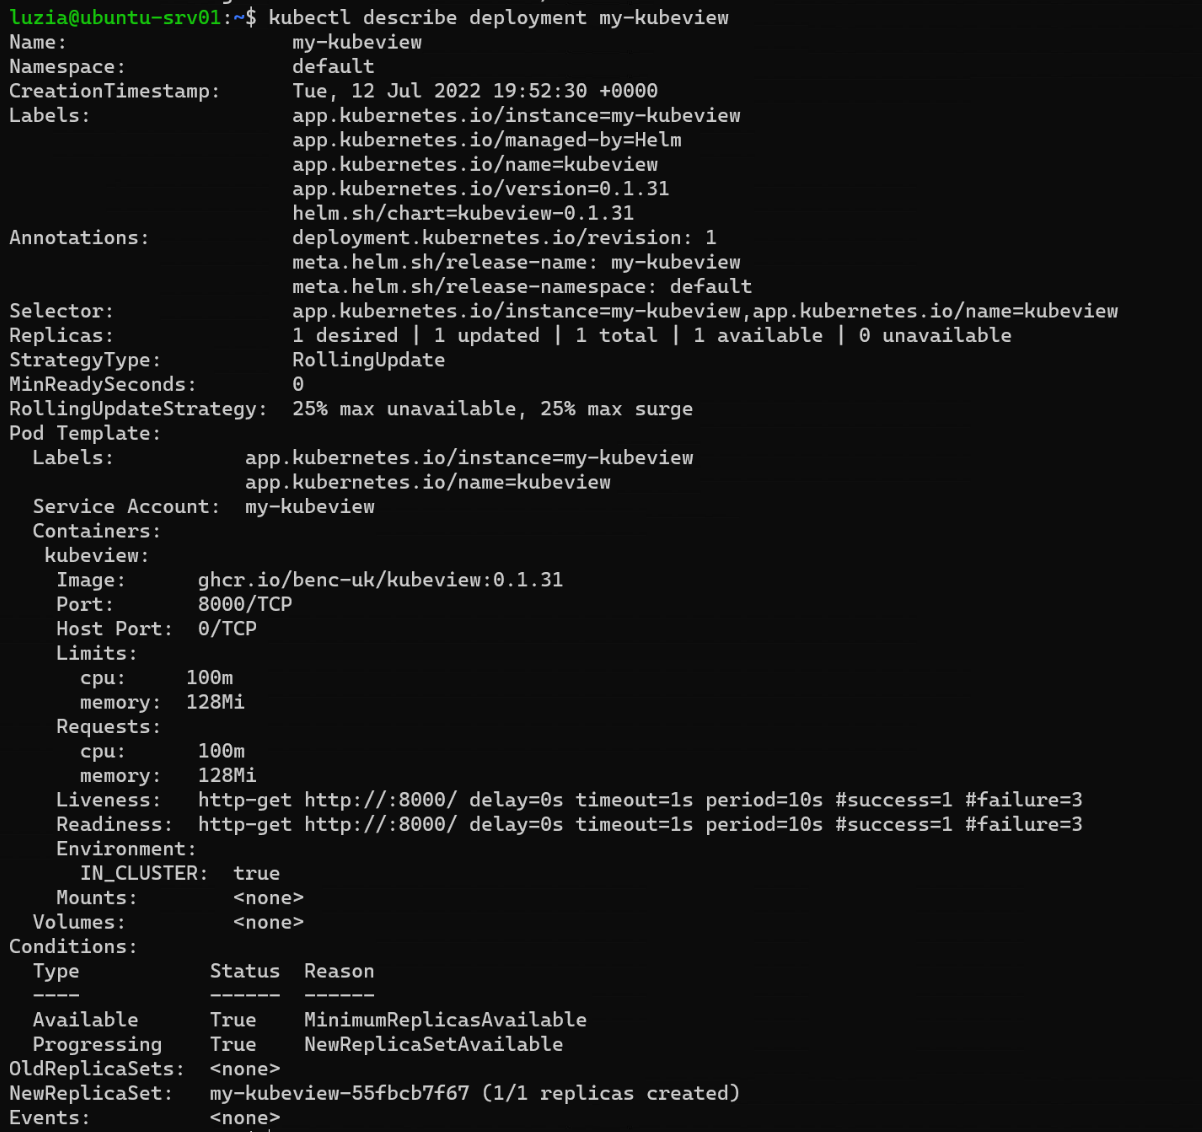
\includegraphics[width=\textwidth]{kubernetes-deployment-details.png}
    \caption{Deployment details}
\end{figure}

\subsection{Rolling Update Strategies}
Applying changes in deployments means changing the number of pods, or even changing every pod to a newer version. 
Exactly how this is done can be defined using Rolling Update Strategies. 

Recent transactions can be viewed, or the last change can be undone with the following commands:

\ttfamily
kubectl rollout history

kubectl rollout undo
\rmfamily

\vspace{3mm}
\noindent
Default Update strategies:

\textbf{Recreate:} Kill all pods and create new ones. Leads to temporary unavailability.

\textbf{RollingUpdate:} updates one pod at a time to guarantee application availability. This behavior can be specified further with Rolling Update Options.

maxUnavailable: limit the number of pods that can be upgraded at the same time

maxSurge: limit the number of pods that can run on top of the specified number to guarantee availability

\subsection{Pod Access Options}

\subsubsection{Service}
An API resource that is used to expose a logical set of pods. A service applies round-robin load-balancing to forward traffic to specific pods. 
To determine which pods are targeted, a label is used as selector. 
Pods are continuously scanned for this label to decide if they should be included in the service.

Services are independent from deployments. All they see is pods with labels, so they can also be used to load-balance between different deployments.

Kube-proxy opens ports on the Cluster IP address for a service and redirects traffic to a pod that matches the specification.

Different Service Types include:

\begin{itemize}
    \item ClusterIP (default): exposes service on an \emph{internal} cluster IP address
    \item NodePort: Allocates a specific port on the node IP, forwarding traffic to a cluster IP address. 
    \item LoadBalancer: \emph{only implemented in public cloud}
    \item ExternalName: \emph{used in migration}
\end{itemize}

\noindent Create services using the commands

\ttfamily kubectl expose deployment \emph{name} --port=\emph{80} \rmfamily 

\noindent or 

\ttfamily kubectl create service --port \rmfamily.

\noindent
This exposes a deployment, allocating its pods as service endpoint.

\vspace{3mm}\noindent
Different port types exist:
\begin{itemize}
    \item targetPort: The port on the container, that the actual application exposes and the service addresses.
    \item port: The port on which the \textbf{service} is accessible.
    \item nodePort: What is \textbf{exposed externally} in the nodePort service type.
\end{itemize}

\subsubsection{Ingress}
Provides external access to internal Kubernetes cluster resources, 
as well as load balancing using an ingress controller (nginx, haproxy, traefik, ...). 

It uses selector labels to connect to pods that are used as a service endpoint. 

It can be configured to do the following:

\begin{itemize}
    \item Give externally reachable URLs to services
    \item Terminate SSL/TLS connections
    \item Offer name-based virtual hosting
    \item Load balance traffic
\end{itemize}

\begin{figure}[h]
    \centering
    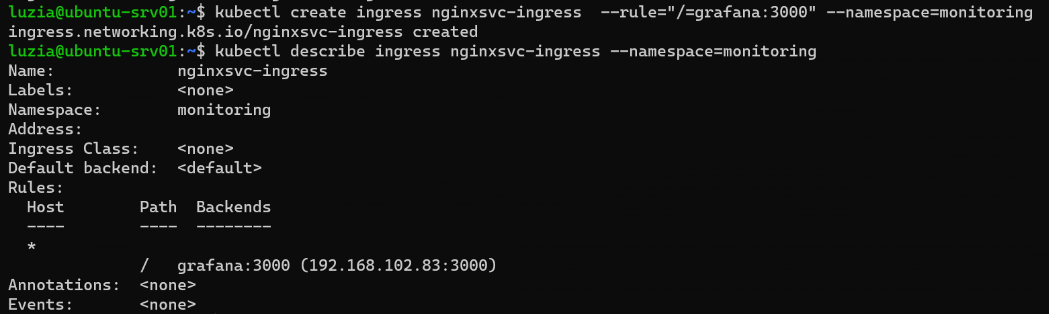
\includegraphics[width=\textwidth]{kubernetes-ingress.png}
\end{figure}

\subsection{Scheduling}

\textbf{Kube-Scheduler:} Matches pods to nodes, is needed to run kubernetes. Labels can be used to influence scheduling (nodeName, nodeSelector, affinity/antiAffinity, taints)

\noindent
\textbf{Filtering:} Nodes need to meet the resources needed to run the pods. 

\emph{PodFitsHostPort, PodFitsResources, PodMatchNodeSelector, CheckNodeDiskPressure, CheckVolumeBinding}

\noindent
\textbf{Scoring:} Ranking after filtering is applied: SelectorSpreadPriority, LeastRequestedPriority, NodeAffinityPriority

\noindent
\textbf{NodeSelector:} Label as Key=Value, can be used in yaml as key: value

\noindent
\textbf{NodeName:} Specify a node host specifically

\noindent
\textbf{Affinity:}
 
nodeAffinity: like nodeSelector, uses labels. Type: required / preferred

podAffinity: required/preferred (+ weight)

\subsection{Taints and Tolerations}

\subsection{Storage}

\subsection{ConfigMaps}

\subsection{Secrets}

\subsection{Probes}

